
%!TEX root = ../thesis.tex
%*******************************************************************************
%****************************** Second Chapter *********************************
%*******************************************************************************

\chapter{Background}

\ifpdf
    \graphicspath{{Chapter2/Figs/Raster/}{Chapter2/Figs/PDF/}{Chapter2/Figs/}}
\else
    \graphicspath{{Chapter2/Figs/Vector/}{Chapter2/Figs/}}
\fi


\fbox{
    \parbox{\textwidth}
    {
        Architecture guidelines for stable Deep Convolutional GANs
        \begin{itemize}
            \item Replace any pooling layers with strided convolutions (discriminator) and fractional-strided convolutions (generator).
            \item Use batchnorm in both the generator and the discriminator.
            \item Remove fully connected hidden layers for deeper architectures.
            \item Use ReLU activation in generator for all layers except for the output, which uses Tanh.
            \item Use LeakyReLU activation in the discriminator for all layers.
        \end{itemize}
    }
}

\pagebreak

\section{Neural Networks}
\subsection{Brain Analogies}

A psychologist, Rosenblatt conceived of the Percetron as a simplified mathematical model of how the neurons in our brains operate: it takes a set of binary inputs (nearby neurons), multiplies each input by a continuous valued weight (the synapse strength to each nearby neuron), and thresholds the sum of these weighted inputs to output a 1 if the sum is big enough and otherwise a 0 (in the same way neurons either fire or do not).

\begin{figure}[H]
\begin{center}
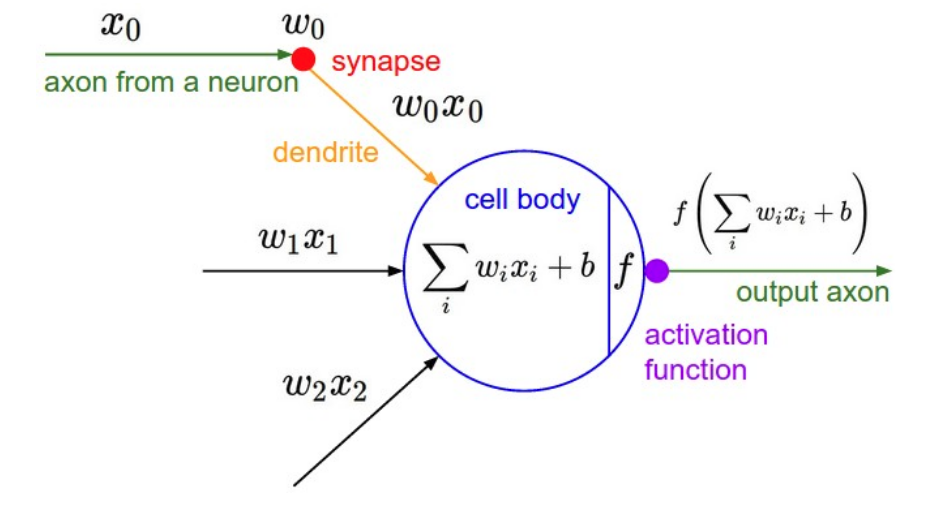
\includegraphics[height=.28\textheight]{Chapter2/Figs/NeuralNetwork.png}
\label{fig:Neural_Network}
\caption{Biologically inspired Neural Network \cite{karparthy}}
\end{center}
\end{figure}

\subsection{Artificial Neural Network}

An Artificial Neural Network (ANN) is an information processing paradigm that is inspired by the way biological nervous systems, such as the brain, process information. The key element of this paradigm is the novel structure of the information processing system. It is composed of a large number of highly interconnected processing elements (neurons) working in unison to solve specific problems. ANNs, like people, learn by example. An ANN is configured for a specific application, such as pattern recognition or data classification, through a learning process. Learning in biological systems involves adjustments to the synaptic connections that exist between the neurons. This is true of ANNs as well.


Neural networks consist of input and output layers, as well as (in most cases) a hidden layer consisting of units that transform the input into something that the output layer can use. They are excellent tools for finding patterns which are far too complex or numerous for a human programmer to extract and teach the machine to recognize.


\begin{figure}[H]
\begin{center}
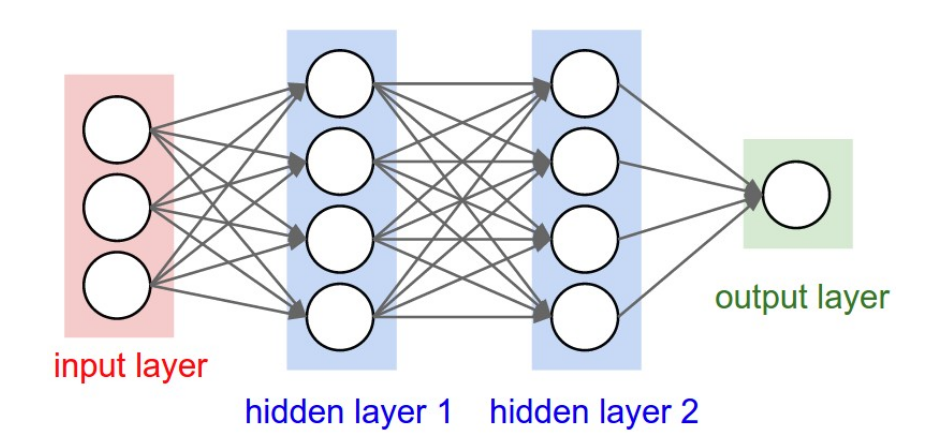
\includegraphics[height=.28\textheight]{Chapter2/Figs/TwoLayeredNN.png}
\label{fig:Two Layered Neural_Network}
\caption{Neural Network with two hidden layers \cite{karparthy}}
\end{center}
\end{figure}


\subsection{Convolutional Neural Network}

“According to the hierarchy model by Hubel and Wiesel, the neural network in the visual cortex has a hierarchy structure: LGB (lateral geniculate body)->simple cells->complex cells->lower order hypercomplex cells->higher order hypercomplex cells. It is also suggested that the neural network between lower order hypercomplex cells and higher order hypercomplex cells has a structure similar to the network between simple cells and complex cells. In this hierarchy, a cell in a higher stage generally has a tendency to respond selectively to a more complicated feature of the stimulus pattern, and, at the same time, has a larger receptive field, and is more insensitive to the shift in position of the stimulus pattern. … Hence, a structure similar to the hierarchy model is introduced in our model.”

Or, more concretely: the first hidden layer of the neural net was convolutional - instead of each neuron having a different weight for each pixel of the input image (40x60=2400 weights), the neurons only have a small set of weights (5x5=25) that were applied a whole bunch of small subsets of the image of the same size. So, for instance instead of having 4 different neurons learn to detect 45 degree lines in each of the 4 corners of the input image, a single neuron could learn to detect 45 degree lines on subsets of the image and do that everywhere within it. Layers past the first work in a similar way, but take in the ‘local’ features found in the previous hidden layer rather than pixel images, and so ‘see’ successively larger portions of the image since they are combining information about increasingly larger subsets of the image. Finally, the last two layers are just plain normal neural net layers that use the higher-order larger features generated by the convolutional layers to determine which digit the input image corresponds to.

The reason for why this is helpful is intuitively if not mathematically clear: without such constraints the network would have to learn the same simple things (such as detecting 45 degree lines, small circles, etc) a whole bunch of times for each portion of the image. But with the constraint there, only one neuron would need to learn each simple feature - and with far fewer weights overall, it could do so much faster! Moreover, since the pixel-exact locations of such features do not matter the neuron could basically skip neighboring subsets of the image - subsampling, now known as a type of pooling - when applying the weights, further reducing the training time. The addition of these two types of layers - convolutional and pooling layers - are the primary distinctions of Convolutional Neural Nets (CNNs/ConvNets) from plain old neural nets.


\section{Probabilistic Machine Learning}
\subsection{Variational Inference}

Given training inputs $\{ \x_1, \hdots, \x_N \}$ and their corresponding outputs $\{\y_1, \hdots, \y_N\}$, in probabilistic modelling we would like to estimate a function $\y = \f(\mathbf{x})$ that is \textit{likely to have generated our outputs}. 
What is a function that is likely to have generated our data? Following the Bayesian approach we would put some \textit{prior} distribution over the space of functions $p(\f)$. This distribution represents our prior belief as to which functions are likely to have generated our data. 
We define a \textit{likelihood} $p(\Y | \f, \X)$ to capture the process in which observations are generated given a specific function.
We then look for the \textit{posterior} distribution over the space of functions given our dataset: $p(\f | \X, \Y)$.
This distribution captures the most likely functions given our observed data.
With it we can predict an output for a new input point $\x^*$ by integrating over all possible functions $\f$,
\begin{align} \label{eq:post}
%p(\f | \X, \Y) \propto p(\Y | \X, \f) p(\f).
p(\y^* | \x^*, \X, \Y) = \int p(\y^* | \f^*) p(\f^* | \x^*, \X, \Y) \td \f^*.
\end{align}

Integral \eqref{eq:post} is intractable for many models. 
To approximate it we could condition the model on a finite set of random variables $\bo$. We make a modelling assumption and assume that the model depends on these variables alone, making them into sufficient statistics in our approximate model.

The predictive distribution for a new input point $\x^*$ is then given by 
$$
p(\y^* | \x^*, \X, \Y) = \int p(\y^* | \f^*) p(\f^* | \x^*, \bo) p(\bo | \X, \Y)\ \td \f^* \td \bo.
$$
The distribution $p(\bo | \X, \Y)$ cannot usually be evaluated analytically as well. Instead we define an approximating \textit{variational} distribution $q(\bo)$, whose structure is easy to evaluate.
We would like our approximating distribution to be as close as possible to the posterior distribution obtained from the original model. We thus minimise the Kullback--Leibler (KL) divergence, intuitively a measure of similarity between two distributions: $\KL(q(\bo) ~||~ p(\bo | \X, \Y))$,
resulting in the approximate predictive distribution 
\begin{align} \label{eq:predictive}
q(\y^* | \x^*) = \int p(\y^* | \f^*) p(\f^* | \x^*, \bo) q(\bo) \td \f^* \td \bo.
\end{align}

Minimising the Kullback--Leibler divergence is equivalent to maximising the \textit{log evidence lower bound},
\begin{align}
&\cL_{\text{VI}} := \int q(\bo) p(\F | \X, \bo) \log p(\Y | \F) \td \F \td \bo - \KL(q(\bo) || p(\bo)) \label{eq:L:VI}
\end{align}
with respect to the variational parameters defining $q(\bo)$. This is known as \textit{variational inference}, a standard technique in Bayesian modelling.
%Note that the KL divergence in the last equation is between the approximate posterior and the \textit{prior} over $\bo$. Maximising this objective will result in a variational distribution $q(\bo)$ that explains the data well (as obtained from the first term---the log likelihood) while still being close to prior---preventing the model from over-fitting.

%Another viewpoint

Variational Bayes is an approximate inference method whereby the posterior $\post$ is approximated by a simpler distribution $\qx \equiv \qpx$ that usually belongs to a parametric family \cite{jordan1999introduction,bishop2006pattern}. The goal of variational inference is to find the variational parameters $\qparams$ for which the variational posterior $\qp$ ``best'' approximates the true posterior. In variational methods, the mismatch between the two distributions is quantified by the Kullback-Leibler (KL) divergence,
\begin{equation} \label{eq:KL}
\text{KL}\left[\qpx || \post\right] = \mathbb{E}_{\qparams} \left[\log \frac{q_{\qparams}(\x)}{\post} \right],
\end{equation}
where we adopted the compact notation $\mathbb{E}_{\qparams} \equiv \mathbb{E}_{q_{\qparams}}$.
Inference is then reduced to an optimization problem, that is finding the variational parameter vector $\qparams$ that minimizes Eq. \ref{eq:KL}. % Using the posterior from Eq. \ref{eq:postandml}, 
We rewrite Eq. \ref{eq:KL} as
\begin{equation} \label{eq:refactoring}
\log \ev = \mathcal{F}[q_{\qparams}] + \text{KL}\left[\qpx || \post\right],
\end{equation}
where
\begin{equation} \label{eq:elbo}
\mathcal{F}\left[ q_{\qparams} \right] =  \mathbb{E}_{\qparams} \left[\log \frac{\like p(\x)}{q_{\qparams}(\x)} \right] = \mathbb{E}_{\qparams} \left[f(\x) \right] + \mathcal{H}[q_{\qparams}(\x)] 
\end{equation}
is the negative free energy, or \emph{evidence lower bound} (ELBO). Here $f(\x) \equiv \log \like p(\x) = \log p(\data, \x)$ is the log joint probability and $\mathcal{H}[q]$ is the entropy of $q$. Note that since the KL divergence is always non-negative, from Eq. \ref{eq:refactoring} we have $\mathcal{F}[q] \le \log \ev$, with equality holding if $\qx \equiv \post$. Thus, maximization of the variational objective, Eq. \ref{eq:elbo}, is equivalent to minimization of the KL divergence, and produces both an approximation of the posterior $\qp$ and a lower bound on the marginal likelihood, which can be used as a metric for model selection.

Normally, $q$ is chosen to belong to a family (e.g., a factorized posterior, or mean field) such that the expected log joint in Eq. \ref{eq:elbo} and the entropy can be computed analytically, possibly providing closed-form equations for a coordinate ascent algorithm. Here, we assume that $f(\x)$, like many computational models of interest, is an expensive black-box function, which prevents a direct computation of Eq. \ref{eq:elbo} analytically or via simple numerical integration.

\subsection{Dropout as Variational Inference}

We now develop approximate variational inference in Bayesian NNs using Bernoulli approximating variational distributions, and relate this to dropout training. This extends on \citep{Gal2015Dropout} as explained in the next section. 

As before, we are interested in finding the most probable functions that have generated our data. In the Bayesian NN case the functions are defined through the NN weights, and these are our sufficient statistics $\bo = (\W_i)_{i=1}^L$. We are thus interested in the posterior over the weights given our observables $\X, \Y$: $p \big( \bo | \X, \Y \big)$. 
This posterior is not tractable for a Bayesian NN, and we use variational inference to approximate it. %(similar techniques have been carried out over the years under different names \citep{hinton1993keeping,
%barber1998ensemble,
%graves2011practical,
%blundell2015weight}). 

To relate the approximate inference in our Bayesian NN to dropout training, we define our approximating variational distribution $q(\W_i)$ for every layer $i$ as 
\begin{align}\label{eq:approx-dist}
\W_i &= \M_i \cdot \diag([\sBb_{i,j}]_{j=1}^{K_i}) \\
\sBb_{i,j} &\sim \text{Bernoulli}(p_i) \text{ for } i = 1, ..., L, ~ j = 1, ..., K_{i-1}. \notag
\end{align}
Here $\sBb_{i,j}$ are Bernoulli distributed random variables with some probabilities $p_i$, and $\M_i$ are variational parameters to be optimised.
The $\diag(\cdot)$ operator maps vectors to diagonal matrices whose diagonals are the elements of the vectors. 

The integral in eq.\ \eqref{eq:L:VI} is intractable and cannot be evaluated analytically for our approximating distribution. Instead, we approximate the integral with Monte Carlo integration over $\bo$. This results in an unbiased estimator for $\cL_{VI}$:
\begin{align}
\widehat{\cL}_{\text{VI}} := \sum_{i=1}^N E \big( \y_i, \widehat{\f} ( \x_i, \widehat{\bo}_i ) \big) - \KL(q(\bo) || p(\bo)) && \widehat{\bo}_i \sim q(\bo)
\end{align}
with $E(\cdot, \cdot)$ being the softmax loss (for a softmax likelihood).
Note that sampling from $q(\W_i)$ is identical to performing dropout on layer $i$ in a network whose weights are $(\M_i)_{i=1}^L$.
The binary variable $\sBb_{i,j} = 0$ corresponds to unit $j$ in layer $i-1$ being dropped out as an input to the $i$'th layer. The second term in eq.\ \eqref{eq:L:VI} can be approximated following \citep{Gal2015Dropout}, resulting in the objective eq.\ \eqref{eq:L:dropout}.
Dropout and Bayesian NNs, in effect, result in the same model parameters that best explain the data.

%In our approximate model $q(\y | \x)$ we have a-priori weight distributions $\N(\bz,\I)$ for every network weight $\W_i$ \citep{Gal2015Dropout}. Our approximate posterior over the weight matrices is $\M_i \diag(\sBb_i)$ with $\sBb_i$ vectors of Bernoulli distributed random variables and variational parameters $\M_i$. 
%Minimising our optimisation objective in eq.\ \eqref{eq:L:GP-MC-reg} maximises the log likelihood term while minimising the KL divergence term. This KL divergence is between the approximate distribution placed over the weights and the prior distribution over the weights. This encourages the model to explain the data well while keeping it from over-fitting.
%The two terms are obtained using a Monte Carlo approximation of the integral over the variational distribution $q(\bo)$. 
Predictions in this model follow equation \eqref{eq:predictive} replacing the posterior $p \big( \bo| \X, \Y \big)$ with the approximate posterior $q \big( \bo \big)$. We can approximate the integral with Monte Carlo integration:
\begin{align} \label{eq:approx_predictive}
p(y^* | \x^*, \X, \Y) \approx 
\int p \big( y^* | \x^*, \bo \big) q \big( \bo \big) 
\td \bo
\approx \frac{1}{T} \sum_{t=1}^T p ( y^* | \x^*, \widehat{\bo}_t )
\end{align}
with $\widehat{\bo}_t \sim q \big( \bo \big)$. This is referred to as MC dropout.

\subsection{Monte  Carlo  variational  inference}
\subsection{Local  reparametrisation  trick}

We utilise the local reparameterization trick \cite{kingma2015variational} and apply it to \acp{cnn}. Following \cite{kingma2015variational,neklyudov2018variance}, we do not sample the weights $w$, but we sample instead layer activations $b$ due to its consequent computational acceleration. The variational posterior probability distribution $q_{\theta}(w_{ijhw}|\mathcal{D})=\mathcal{N}(\mu_{ijhw},\alpha_{ijhw}\mu^2_{ijhw})$ (where $i$ and $j$ are the input, respectively output layers, $h$ and $w$ the height, respectively width of any given filter) allows to implement the local reparamerization trick in convolutional layers. This results in the subsequent equation for convolutional layer activations $b$:
\begin{equation}
    b_j=A_i\ast \mu_i+\epsilon_j\odot \sqrt{A^2_i\ast (\alpha_i\odot \mu^2_i)}
\end{equation}
where $\epsilon_j \sim \mathcal{N}(0,1)$, $A_i$ is the receptive field, $\ast$ signalises the convolutional operation, and $\odot$ the component-wise multiplication.

\section{Bayesian Uncertainities}

There are two major types of uncertainty one can model. \textit{Aleatoric} uncertainty captures noise inherent in the observations. On the other hand, \textit{epistemic} uncertainty accounts for uncertainty in the model -- uncertainty which can be explained away given enough data. Traditionally it has been difficult to model epistemic uncertainty in computer vision, but with new Bayesian deep learning tools this is now possible.
We study the benefits of modeling epistemic vs.\ aleatoric uncertainty in Bayesian deep learning models for vision tasks. For this we present a Bayesian deep learning framework combining input-dependent aleatoric uncertainty together with epistemic uncertainty. We study models under the framework with per-pixel semantic segmentation and depth regression tasks. Further, our explicit uncertainty formulation leads to new loss functions for these tasks, which can be interpreted as learned attenuation. This makes the loss more robust to noisy data, also giving new state-of-the-art results on segmentation and depth regression benchmarks. 

In Bayesian modeling, there are two main types of uncertainty one can model \citep{der2009aleatory}. \textit{Aleatoric} uncertainty captures noise inherent in the observations.
% , also known as \textit{risk}. 
This could be for example sensor noise or motion noise, resulting in uncertainty which cannot be reduced even if more data were to be collected.
On the other hand, \textit{epistemic} uncertainty accounts for uncertainty in the model parameters -- uncertainty which captures our ignorance about which model generated our collected data. 
This uncertainty can be explained away given enough data, and is often referred to as \textit{model uncertainty}. Aleatoric uncertainty can further be categorized into \textit{homoscedastic} uncertainty, uncertainty which stays constant for different inputs, and \textit{heteroscedastic} uncertainty. Heteroscedastic uncertainty depends on the inputs to the model, with some inputs potentially having more noisy outputs than others. 
Heteroscedastic uncertainty is especially important for computer vision applications. For example, for depth regression, highly textured input images with strong vanishing lines are expected to result in confident predictions, whereas an input image of a featureless wall is expected to have very high uncertainty.


Existing approaches to Bayesian deep learning capture either epistemic uncertainty alone, or aleatoric uncertainty alone \cite{gal2016thesis}. These uncertainties are formalised as probability distributions over either the model parameters, or model outputs, respectively. Epistemic uncertainty is modeled by placing a prior distribution over a model's weights, and then trying to capture how much these weights vary given some data. Aleatoric uncertainty on the other hand is modeled by placing a distribution over the output of the model. For example, in regression our outputs might be modeled as corrupted with Gaussian random noise. In this case we are interested in learning the noise's variance as a function of different inputs (such noise can also be modeled with a constant value for all data points, but this is of less practical interest). These uncertainties, in the context of Bayesian deep learning, are explained in more detail in this section. 

\section{Bayes by Backprop}
\textit{Bayes by Backprop} \cite{graves2011practical, blundell2015weight} is a variational inference method to learn the posterior distribution on the weights $w \sim q_{\theta}(w|\mathcal{D})$ of a neural network from which weights $w$ can be sampled in backpropagation. 
It regularises the weights by minimising a compression cost, known as the variational free energy or the expected lower bound on the marginal likelihood.

Since the true posterior is typically intractable, an approximate distribution $q_{\theta}(w|\mathcal{D})$ is defined that is aimed to be as similar as possible to the true posterior $p(w|\mathcal{D})$, measured by the Kullback-Leibler (KL) divergence \cite{kullback1951information}. Hence, we define the optimal parameters $\theta^{opt}$ as
\begin{equation}
    \begin{aligned} \label{KL}
        \theta^{opt}&=\underset{\theta}{\text{arg min}}\ \text{KL} \ [q_{\theta}(w|\mathcal{D})\|p(w|\mathcal{D})] \\
        &=\underset{\theta}{\text{arg min}}\ \text{KL} \ [q_{\theta}(w|\mathcal{D})\|p(w)] \\ & -\mathbb{E}_{q(w|\theta)}[\log p(\mathcal{D}|w)]+\log p(\mathcal{D})
    \end{aligned}
\end{equation}

where
\begin{equation}
    \text{KL} \ [q_{\theta}(w|\mathcal{D})\|p(w)]= \int q_{\theta}(w|\mathcal{D})\log\frac{q_{\theta}(w|\mathcal{D})}{p(w)}dw .
\end{equation}
This derivation forms an optimisation problem with a resulting cost function widely known as \textit{variational free energy} \cite{neal1998view,yedidia2005constructing,friston2007variational} which is built upon two terms: the former, $\text{KL} \ [q_{\theta}(w|\mathcal{D})\|p(w)]$, is dependent on the definition of the prior $p(w)$, thus called complexity cost, whereas the latter, $\mathbb{E}_{q(w|\theta)}[\log p(\mathcal{D}|w)]$, is dependent on the data $p(\mathcal{D}|w)$, thus called likelihood cost. 
The term $\log p(\mathcal{D})$ can be omitted in the optimisation because it is constant.
\newline Since the KL-divergence is also intractable to compute exactly, we follow a stochastic variational method \cite{graves2011practical,blundell2015weight}.
We sample the weights $w$ from the variational distribution $q_{\theta}(w|\mathcal{D})$ since it is much more probable to draw samples which are appropriate for numerical methods from the variational posterior $q_{\theta}(w|\mathcal{D})$ than from the true posterior $p(w|\mathcal{D})$. Consequently, we arrive at the tractable cost function \eqref{cost} which is aimed to be optimized, i.e. minimised w.r.t. $\theta$, during training:
\begin{equation} \label{cost}
    \mathcal{F}(\mathcal{D}, \theta)\approx \sum_{i=1}^n \log q_{\theta}(w^{(i)}|\mathcal{D})-\log p(w^{(i)})-\log p(\mathcal{D}|w^{(i)})
\end{equation}
%
where $n$ is the number of draws.
\newline We sample $w^{(i)}$ from $q_{\theta}(w|\mathcal{D})$. The uncertainty afforded by \textit{Bayes by Backprop} trained neural networks has been used successfully for training feedforward neural networks in both supervised and reinforcement learning environments \cite{blundell2015weight,lipton2016efficient,houthooft2016curiosity}, for training recurrent neural networks \cite{fortunato2017bayesian}, but has not been applied to convolutional neural networks to-date.

